\documentclass[DIV         = 14,
               fontsize    = 10,
               index       = totoc,
               twoside,
               cadre,
               headings    = small
               ]{tkz-doc}
%\setmainlanguage{english}
%\usepackage[match]{luatexja-fontspec}
%\usepackage{polyglossia}
%\newfontfamily\chinesefont{FandolSong}
\gdef\tkznameofpack{Geometry}
\gdef\tkzversionofpack{1.0a}
\gdef\tkzdateofpack{\today}
\gdef\tkznameofdoc{doc-mathematics}
\gdef\tkzversionofdoc{1.0a} 
\gdef\tkzdateofdoc{\today}
\gdef\tkzauthorofpack{Zhifeng Zhang}
\gdef\tkzadressofauthor{}
\gdef\tkznamecollection{Algebra}
\gdef\tkzurlauthor{https://blackgolfer.github.io/geometry}
\gdef\tkzengine{lualatex}
\gdef\tkzurlauthorcom{https://blackgolfer.github.io/geometry}
\nameoffile{\tkznameofpack}
% -- Packages ---------------------------------------------------          
\usepackage[dvipsnames,svgnames]{xcolor}
\usepackage{calc}
\usepackage{tkz-base} 
\usepackage[lua]{tkz-euclide} 
\usepackage{pgfornament} 
\usetikzlibrary{backgrounds}
\usepackage[colorlinks,pdfencoding=auto, psdextra]{hyperref}
\hypersetup{
      linkcolor=Gray,
      citecolor=Green,
      filecolor=Mulberry,
      urlcolor=NavyBlue,
      menucolor=Gray,
      runcolor=Mulberry,
      linkbordercolor=Gray,
      citebordercolor=Green,
      filebordercolor=Mulberry,
      urlbordercolor=NavyBlue,
      menubordercolor=Gray,
      runbordercolor=Mulberry,
      pdfsubject={Geometry},
      pdfauthor={\tkzauthorofpack},
      pdftitle={\tkznameofpack},
      pdfcreator={\tkzengine}
}
\usepackage{tkzexample}
\linespread{1.05}      % Pagella needs more space between lines
\let\rmfamily\ttfamily
\usepackage{multicol,lscape}
\usepackage[english]{babel}
\usepackage[normalem]{ulem}
\usepackage{byrne}
\usepackage{listings}
\usepackage{multirow,multido,booktabs,cellspace}
\usepackage{shortvrb,fancyvrb,bookmark} 
\usepackage{makeidx}
\makeindex 

%<---------------------------------------------------------------------------> 
% tikz
\usetikzlibrary{shapes.geometric}

%<---------------------------------------------------------------------------> 
% settings styles
\tkzSetUpColors[background=white,text=black]  
\tkzSetUpCompass[color=orange, line width=.2pt,delta=10]
\tkzSetUpArc[color=gray,line width=.2pt]
\tkzSetUpPoint[size=2,color=teal]
\tkzSetUpLine[line width=.2pt,color=teal]
\tkzSetUpStyle[color=orange,line width=.2pt]{new}
\tikzset{every picture/.style={line width=.2pt}}
\tikzset{label angle style/.append style={color=teal,font=\footnotesize}} 
\tikzset{label style/.append style={below,color=teal,font=\scriptsize}}
\tikzset{new/.style={color=orange,line width=.2pt}} 

\pgfdeclarelayer{background layer}
\pgfsetlayers{background layer,main}
\tikzset{old paper/.style={%
execute at end picture={%
\begin{pgfonlayer}{background layer} 
\clip (current bounding box.south west) rectangle (current bounding box.north east);
\node[inner sep=0pt] (p) at (current bounding box.center)
     {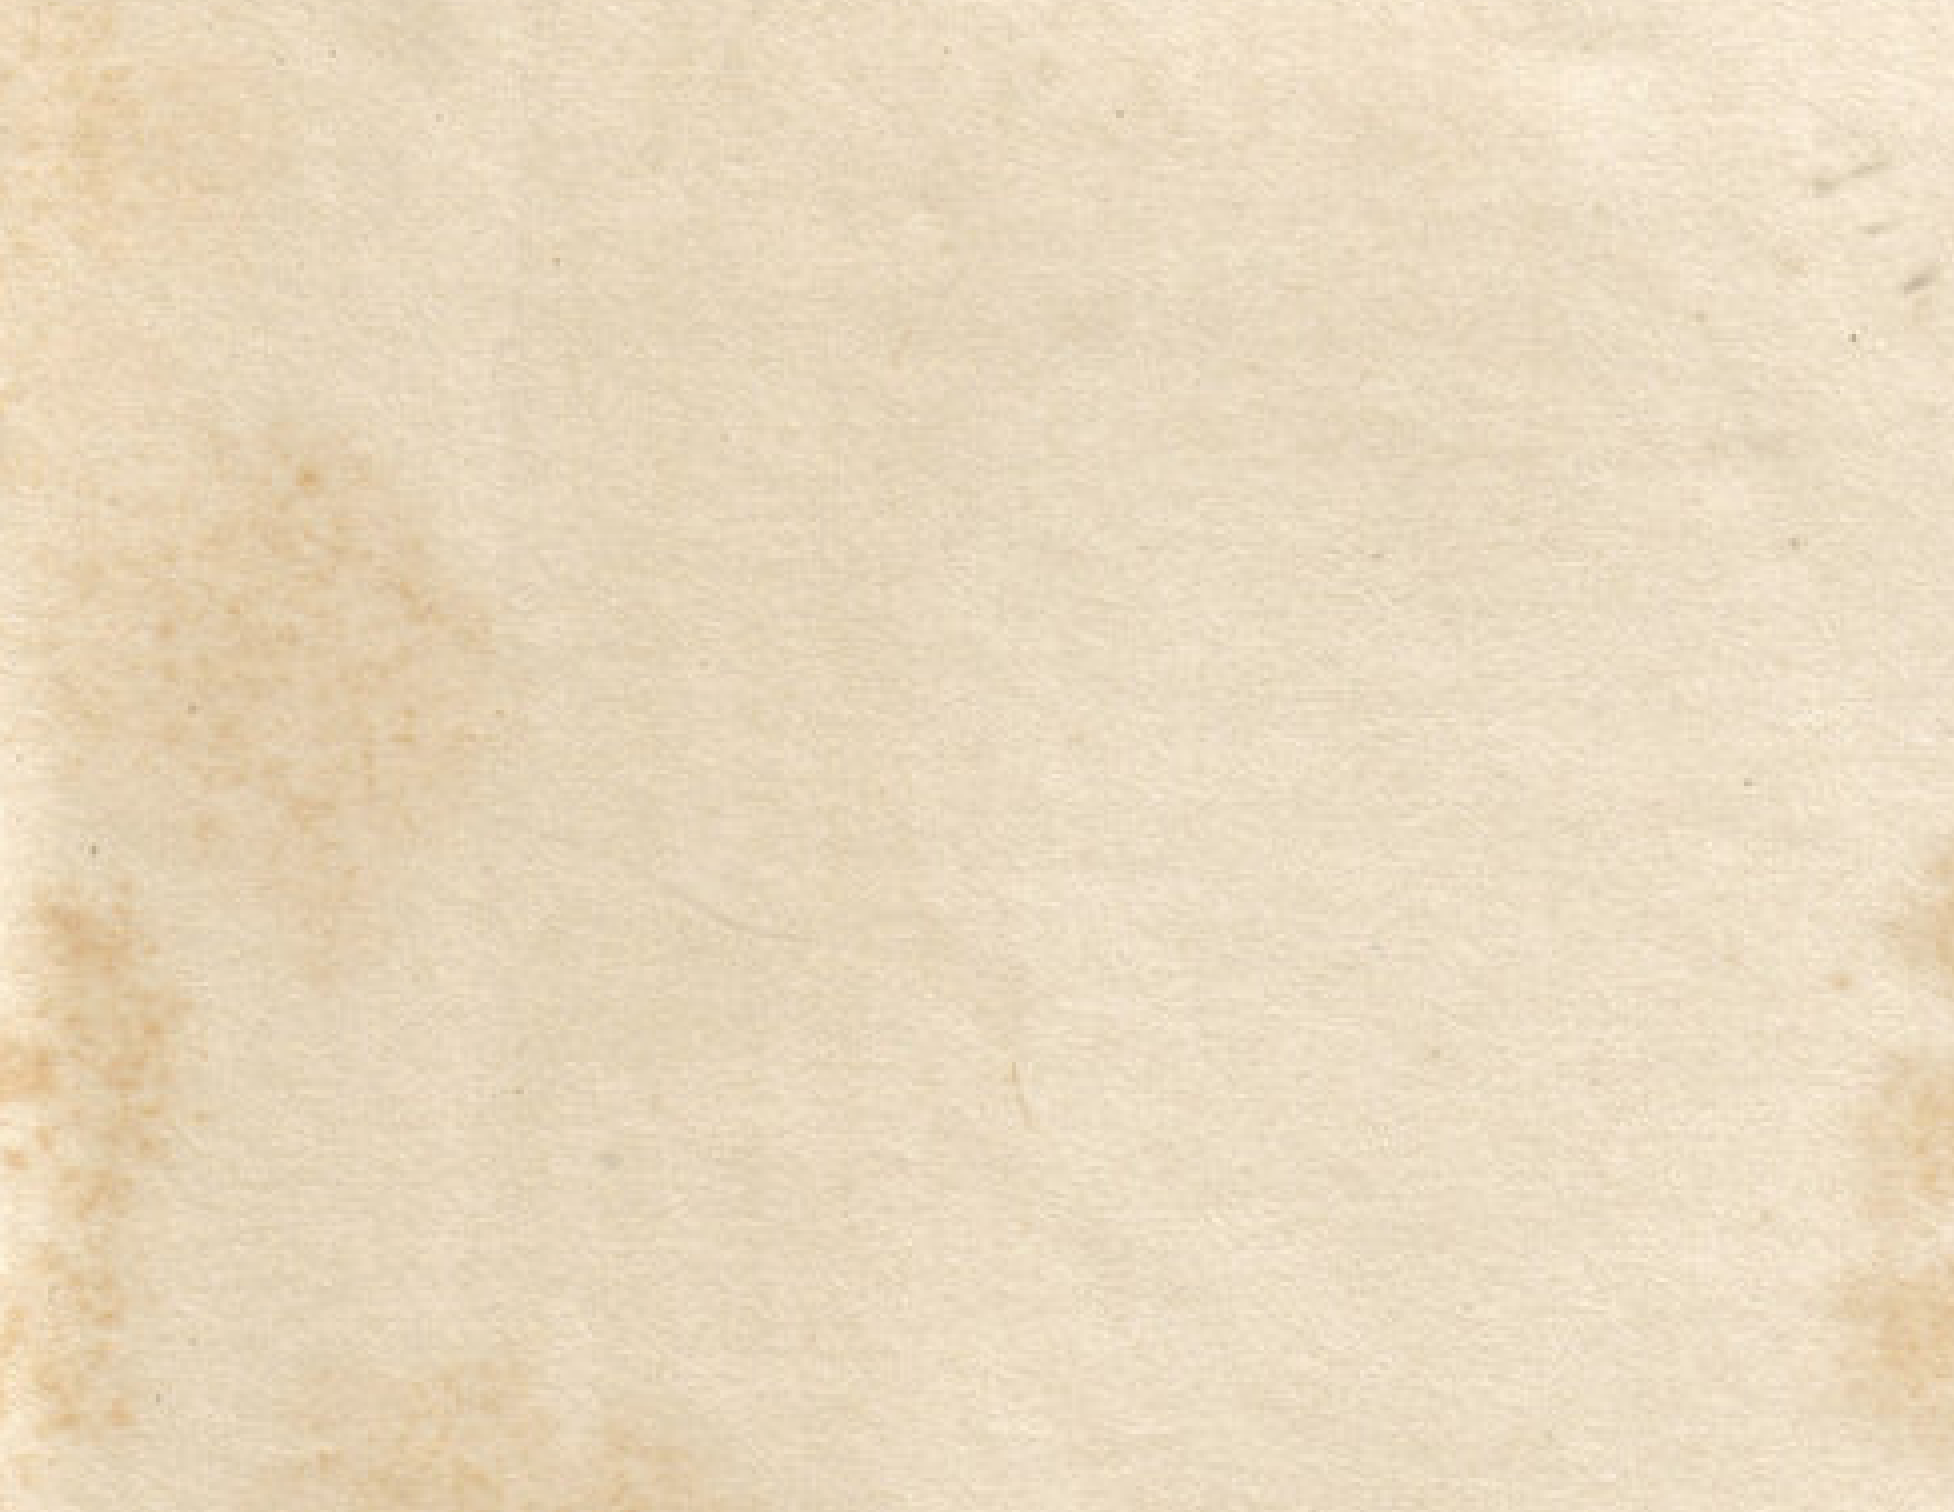
\includegraphics{old_paper.png}};
\end{pgfonlayer}%
}}}

%<--------------------------------------------------------------------------->
% setting metapost
\lstset{
language=MetaPost,
alsolanguage=TeX,
numbers=none,
basicstyle=\ttfamily\scriptsize
}
\def\mpPre{textLabels := true;}

%<--------------------------------------------------------------------------->
% new commands
\usepackage{colortbl}
\usepackage{nccmath}
\newcommand{\defbox}[2][]%
{

\begin{tikzpicture}
  \node [mybox,title={#1}] (box){%
      \begin{minipage}{0.90\textwidth}
        {\emph{
          #2
        }} 
      \end{minipage}
  };
\end{tikzpicture}% 
}
\newtheorem{definition}{Definition}
\newtheorem{theorem}{Theorem}
\newtheorem{corollary}{Corollary}
\newtheorem{proposition}{Proposition}
\newtheorem{lemma}{Lemma}

\AtBeginDocument{\MakeShortVerb{\|}} % link to shortvrb

\begin{document}

\parindent=0pt
\tkzTitleFrame{Reflection and Coxeter Group}
\clearpage

\clearpage
\tableofcontents

\clearpage
\newpage

\part{Reflection Group}
\section{Permutation Group}
A \textit{permutation group} is a group $G$ whose elements are permutations of a given set $M$ and whose group
operation is the composition of permutations in G (which are thought of as bijective functions from the set $M$
to itself). The group of all permutations of a set $M$ is the \textit{symmetric group} of $M$, often written as
$Sym(M)$. The term permutation group thus means a subgroup of the symmetric group. If $M=\{1, 2, ..., n\}$ then
$Sym(M)$ is usually denoted by $S_n$, and may be called the symmetric group on $n$ letters.

By Cayley's theorem, every group is isomorphic to some permutation group.

The way in which the elements of a permutation group permute the elements of the set is called its group action.

\subsection{Symmetric group}
Being a subgroup of a symmetric group, all that is necessary for a set of permutations to satisfy the group
axioms and be a permutation group is that it contain the identity permutation, the inverse permutation of each
permutation it contains, and be closed under composition of its permutations. A general property of finite
groups implies that a finite nonempty subset of a symmetric group is again a group if and only if it is closed
under the group operation.

The \textit{degree} of a group of permutations of a finite set is the number of elements in the set.
The \textit{order} of a group (of any type) is the number of elements (cardinality) in the group. By Lagrange's
theorem, the order of any finite permutation group of degree $n$ must divide $n!$ since $n$-factorial is the
order of the symmetric group $S_n$.

\subsection{Permutation}
\subsubsection{Notations}
Since permutations are bijections of a set, they can be represented by Cauchy's two-line notation. This notation
lists each of the elements of $M$ in the first row, and for each element, its image under the permutation below
it in the second row.  If $\sigma$  is a permutation of the set $M=\{x_{1},x_{2},\ldots ,x_{n}\}$ then,
$$\sigma =
    {
    \begin{pmatrix}
        x_{1} & x_{2} & x_{3} & \cdots & x_{n} \\\sigma (x_{1})&\sigma (x_{2})&\sigma (x_{3})&\cdots &\sigma (x_{n})
    \end{pmatrix}
    }.
$$
For instance, a particular permutation of the set $\{1, 2, 3, 4, 5\}$ can be written as
$$\sigma ={\begin{pmatrix}1&2&3&4&5\\2&5&4&3&1\end{pmatrix}};$$
this means that $\sigma$ satisfies $\sigma(1) = 2$, $\sigma(2) = 5$, $\sigma(3) = 4$,
$\sigma(4) = 3$, and $\sigma(5) = 1$. The elements of M need not appear in any special order in the first row,
so the same permutation could also be written as
$$\sigma ={\begin{pmatrix}3&2&5&1&4\\4&5&1&2&3\end{pmatrix}}.$$
Permutations are also often written in cycle notation (cyclic form) so that given the set $M = \{1, 2, 3, 4\}$,
a permutation $g$ of $M$ with $g(1) = 2$, $g(2) = 4$, $g(4) = 1$ and $g(3) = 3$ will be written as
$(1, 2, 4)(3)$, or more commonly, $(1, 2, 4)$ since $3$ is left unchanged; if the objects are denoted by
single letters or digits, commas and spaces can also be dispensed with, and we have a notation such as $(124)$.
The permutation written above in 2-line notation would be written in cycle notation as $\sigma=(125)(34)$.

\subsubsection{Composition of permutations - the group product}
The product of two permutations is defined as their composition as functions, so
$\displaystyle \sigma \cdot \pi$ is the function that maps any element x of the set to
$\displaystyle \sigma (\pi (x))$. Note that the rightmost permutation is applied to the argument first,
because of the way function composition is written. Some authors prefer the leftmost factor acting first,
but to that end permutations must be written to the right of their argument, often as a superscript,
so the permutation $\sigma$  acting on the element $x$ results in the image
$\displaystyle x^{\sigma }$. With this convention, the product is given by
$\displaystyle x^{\sigma \cdot \pi }=(x^{\sigma })^{\pi }$. However, this gives a different rule for
multiplying permutations. This convention is commonly used in the permutation group literature, but
we use the convention where the rightmost permutation is applied first.

Since the composition of two bijections always gives another bijection, the product of two permutations is
again a permutation. In two-line notation, the product of two permutations is obtained by rearranging the
columns of the second (leftmost) permutation so that its first row is identical with the second row of the
first (rightmost) permutation. The product can then be written as the first row of the first permutation over
the second row of the modified second permutation. For example, given the permutations,

$$P=
    \begin{pmatrix}1&2&3&4&5\\2&4&1&3&5\end{pmatrix}\quad {\text{ and }}\quad
    Q={\begin{pmatrix}1&2&3&4&5\\5&4&3&2&1\end{pmatrix}},
$$
the product QP is:
$$
    QP=
    \begin{pmatrix}
        1&2&3&4&5\\5&4&3&2&1\end{pmatrix}{\begin{pmatrix}1 & 2 & 3 & 4 & 5 \\2&4&1&3&5
    \end{pmatrix}}
    =
    \begin{pmatrix}2&4&1&3&5\\4&2&5&3&1\end{pmatrix}
    \begin{pmatrix}1&2&3&4&5\\2&4&1&3&5\end{pmatrix}
    =
    \begin{pmatrix}1&2&3&4&5\\4&2&5&3&1\end{pmatrix}.
$$
The composition of permutations, when they are written in cycle notation, is obtained by juxtaposing the two
permutations (with the second one written on the left) and then simplifying to a disjoint cycle form if desired.
Thus, the above product would be given by:
$$Q\cdot P=(15)(24)\cdot (1243)=(1435).$$
This can be worked out as follows: Write the cycles next to each other and compute the image of
each $x\in\{1,2,3,4,5\}$ by applying the cycles one at a time going from right to left:
$$
    \begin{array}{lllll}
        Q\cdot P(1) & = & _4(15)_4(24)_2(1243)_1 & = & 4  \\
        Q\cdot P(2) & = & _2(15)_2(24)_4(1243)_2 & = & 2  \\
        Q\cdot P(3) & = & _5(15)_1(24)_1(1243)_3 & = & 5  \\
        Q\cdot P(4) & = & _3(15)_3(24)_3(1243)_4 & = & 3  \\
        Q\cdot P(5) & = & _1(15)_5(24)_5(1243)_5 & = & 1.
    \end{array}
$$
Since function composition is associative, so is the product operation on permutations:
$\displaystyle (\sigma \cdot \pi )\cdot \rho =\sigma \cdot (\pi \cdot \rho )$. Therefore, products of two or
more permutations are usually written without adding parentheses to express grouping; they are also usually
written without a dot or other sign to indicate multiplication (the dots of the previous example were added for
emphasis, so would simply be written as $\displaystyle \sigma \pi \rho $).

\subsubsection{Transposition}
\begin{definition}[Transposition]
    A \textit{transposition} is a $2$-cycle $(ab)$.
\end{definition}
\begin{definition}[Simple transposition]
    A \textit{simple transposition} (also called simple reflection) is a transposition with consecutive letters:
    $$s_i:=(i,i+1).$$
\end{definition}
In the group of permutations of $n+1$ letters there are n simple reflections:
$s_1=(12),\ s_2=(23),\ \dots\ ,\ s_n=(n,n+1)$.

\begin{theorem}
    A permutation $f$ can be written as a product of simple reflections.
\end{theorem}

\begin{definition}
    Suppose that $f$ is a permutation of the letters $1, 2, \dots , n+1$. Then the length $\ell(f)$ of $f$
    is defined to be the number of pairs of integers $i, j$ so that
    \begin{enumerate}
        \item $1\leq i<j\leq n+1$
        \item $f(i) > f(j)$.
    \end{enumerate}
    In other words, it is the number of pairs of numbers whose order is switched by $f$.
\end{definition}

\begin{corollary}
    Any permutation $f$ can be written as a product of $\ell(f)$ simple reflections.
\end{corollary}

Example: $(25673)(14)$
\begin{enumerate}
    \item First get the Cauchy's notation: 
        $$
        \begin{pmatrix}
            1&2&3&4&5&6&7\\
            4&5&2&1&6&7&3
        \end{pmatrix}
        $$
    \item Run the bubble sort on $(4521673)$:
        $$
        \begin{array}{ccccccccc}
            (4521673)&\underset{23}{\longrightarrow}&(4251673)&\underset{34}{\longrightarrow}&(4215673)
            &\underset{12}{\longrightarrow}&(2415673)&\underset{23}{\longrightarrow}&(2145673)\\
            &\underset{12}{\longrightarrow}&(1245673)&\underset{67}{\longrightarrow}&(1245637)
            &\underset{56}{\longrightarrow}&(1245367)&\underset{45}{\longrightarrow}&(1243567)\\
            &\underset{34}{\longrightarrow}&(1234567)
        \end{array}
        $$
\end{enumerate}
This leads to the result: $(25673)(14)=(34)(45)(56)(67)(12)(23)(12)(34)(23)=s_3s_4s_5s_6s_1s_2s_1s_3s_2$.
We can calculate each element in $\{1,2,3,4,5,6,7\}$ to verify:
$$
\begin{array}{ccc}
    (34)(45)(56)(67)(12)(23)(12)(34)(23)(1)&=&4\\
    (34)(45)(56)(67)(12)(23)(12)(34)(23)(2)&=&5\\
    (34)(45)(56)(67)(12)(23)(12)(34)(23)(3)&=&2\\
    (34)(45)(56)(67)(12)(23)(12)(34)(23)(4)&=&1\\
    (34)(45)(56)(67)(12)(23)(12)(34)(23)(5)&=&6\\
    (34)(45)(56)(67)(12)(23)(12)(34)(23)(6)&=&7\\
    (34)(45)(56)(67)(12)(23)(12)(34)(23)(7)&=&3
\end{array}
$$


\subsubsection{Neutral element and inverses}
The identity permutation, which maps every element of the set to itself, is the neutral element for this product.
In two-line notation, the identity is
$$\begin{pmatrix}1&2&3&\cdots &n\\1&2&3&\cdots &n\end{pmatrix}.$$
In cycle notation, $e=(1)(2)(3)\dots(n)$ which by convention is also denoted by just $(1)$ or even $()$.

Since bijections have inverses, so do permutations, and the inverse $\sigma^{-1}$ of $\sigma$ is again a
permutation. Explicitly, whenever $\sigma(x)=y$ one also has $\sigma^{-1}(y)=x$. In two-line notation the inverse
can be obtained by interchanging the two lines (and sorting the columns if one wishes the first line to be in a
given order). For instance
$$
    \begin{pmatrix}1&2&3&4&5\\2&5&4&3&1\end{pmatrix}^{-1}
    =\begin{pmatrix}2&5&4&3&1\\1&2&3&4&5\end{pmatrix}
    =\begin{pmatrix}1&2&3&4&5\\5&1&4&3&2\end{pmatrix}.
$$
To obtain the inverse of a single cycle, we reverse the order of its elements. Thus,
$$(125)^{-1}=(521)=(152).$$
To obtain the inverse of a product of cycles, we first reverse the order of the cycles, and then we take the
inverse of each as above. Thus,
$$[(125)(34)]^{-1}=(34)^{-1}(125)^{-1}=(43)(521)=(34)(152).$$
Having an associative product, an identity element, and inverses for all its elements, makes the set of all
permutations of $M$ into a group, $Sym(M)$; a permutation group.

\subsubsection{Examples}
Consider the following set $G_1$ of permutations of the set $M = \{1, 2, 3, 4\}$:
\begin{itemize}
    \item $e = (1)(2)(3)(4) = (1)$
          This is the identity, the trivial permutation which fixes each element.
    \item $a = (1 2)(3)(4) = (1 2)$
          This permutation interchanges $1$ and $2$, and fixes $3$ and $4$.
    \item $b = (1)(2)(3 4) = (3 4)$
          Like the previous one, but exchanging $3$ and $4$, and fixing the others.
    \item $ab = (1 2)(3 4)$
          This permutation, which is the composition of the previous two, exchanges simultaneously $1$ with $2$,
          and $3$ with $4$.
\end{itemize}
$G_1$ forms a group, since $aa = bb = e$, $ba = ab$, and $abab = e$. This permutation group is,
as an abstract group, the Klein group $V_4$.

As another example consider the group of symmetries of a square. Let the vertices of a square be
labeled $1$, $2$, $3$ and $4$ (counterclockwise around the square starting with 1 in the top left corner).
The symmetries are determined by the images of the vertices, that can, in turn, be described by permutations.
The rotation by $90^\circ$ (counterclockwise) about the center of the square is described by the permutation
$(1234)$. The $180^\circ$ and $270^\circ$ rotations are given by $(13)(24)$ and $(1432)$, respectively.
The reflection about the horizontal line through the center is given by $(12)(34)$ and the corresponding
vertical line reflection is $(14)(23)$. The reflection about the $1,3$−diagonal line is $(24)$ and reflection
about the $2,4$−diagonal is $(13)$. The only remaining symmetry is the identity $(1)(2)(3)(4)$.
This permutation group is known, as an abstract group, as the \textit{dihedral group} of order $8$.

\subsection{Group actions}
In the above example of the symmetry group of a square, the permutations "describe" the movement of the vertices
of the square induced by the group of symmetries. It is common to say that these group elements are "acting" on
the set of vertices of the square. This idea can be made precise by formally defining a \textbf{group action}.

Let $G$ be a group and $M$ a nonempty set. An action of $G$ on $M$ is a function $f: G\times M\rightarrow M$
such that
\begin{itemize}
    \item $f(1, x) = x$, for all $x\in M$ ($1$ is the identity (neutral) element of the group $G$), and
    \item $f(g, f(h, x)) = f(gh, x)$, for all $g,h\in G$ and all $x\in M$.
\end{itemize}
This pair of conditions can also be expressed as saying that the action induces a group homomorphism from $G$
into $Sym(M)$. Any such homomorphism is called a (permutation) representation of $G$ on $M$.

For any permutation group, the action that sends $(g, x)\rightarrow g(x)$ is called the natural action of $G$
on $M$. This is the action that is assumed unless otherwise indicated. In the example of the symmetry group of
the square, the group's action on the set of vertices is the natural action. However, this group also induces
an action on the set of four triangles in the square, which are: $t_1 = 234$, $t_2 = 134$, $t_3 = 124$ and
$t_4 = 123$. It also acts on the two diagonals: $d_1 = 13$ and $d_2 = 24$.
\vskip 1em
\begin{tabular}{lll}
    \toprule
    \rowcolor{Gainsboro!60}
    Group element & Action on triangles  & Action on diagonals \\
    \midrule
    $(1)$         & $(1)$                & $(1)$               \\
    $(1234)$      & $(t_1 t_2 t_3 t_4)$  & $(d_1 d_2)$         \\
    $(13)(24)$    & $(t_1 t_3)(t_2 t_4)$ & $(1)$               \\
    $(1432)$      & $(t_1 t_4 t_3 t_2)$  & $(d_1 d_2)$         \\
    $(12)(34)$    & $(t_1 t_2)(t_3 t_4)$ & $(d_1 d_2)$         \\
    $(14)(23)$    & $(t_1 t_4)(t_2 t_3)$ & $(d_1 d_2)$         \\
    $(13)$        & $(t_1 t_3)$          & $(1)$               \\
    $(24)$        & $(t_2 t_4)$          & $(1)$
\end{tabular}

\subsubsection{Transitive actions}
The action of a group $G$ on a set $M$ is said to be transitive if, for every two elements $s$, $t$ of $M$,
there is some group element $g$ such that $g(s) = t$. Equivalently, the set $M$ forms a single orbit under the
action of $G$. Of the examples above, the group $\{e, (1 2), (3 4), (1 2)(3 4)\}$ of permutations of
$\{1, 2, 3, 4\}$ is not transitive (no group element takes $1$ to $3$) but the group of symmetries of
a square is transitive on the vertices.

\subsubsection{Primitive actions}
A permutation group $G$ acting transitively on a non-empty finite set $M$ is \textit{imprimitive} if there is
some nontrivial set partition of $M$ that is preserved by the action of $G$, where ``nontrivial" means that
the partition isn't the partition into singleton sets nor the partition with only one part. Otherwise,
if $G$ is transitive but does not preserve any nontrivial partition of M, the group $G$ is \textit{primitive}.

For example, the group of symmetries of a square is imprimitive on the vertices: if they are numbered
$1, 2, 3, 4$ in cyclic order, then the partition $\{{1, 3}, {2, 4}\}$ into opposite pairs is preserved by
every group element. On the other hand, the full symmetric group on a set $M$ is always primitive.

\subsection{Cayley's theorem}
\defbox[Cayley's theorem]{
    Any group $G$ can act on itself (the elements of the group being thought of as the set $M$) in many ways.
    In particular, there is a regular action given by (left) multiplication in the group. That is, $f(g,x)=gx$
    for all $g$ and $x$ in $G$. For each fixed $g$, the function $fg(x)=gx$ is a bijection on $G$ and
    therefore a permutation of the set of elements of $G$. Each element of $G$ can be thought of as a
    permutation in this way and so $G$ is isomorphic to a permutation group.
}

For example, consider the group $G_1$ acting on the set $\{1, 2, 3, 4\}$ given above. Let the elements of
this group be denoted by $e$, $a$, $b$ and $c = ab = ba$. The action of $G_1$ on itself described in
Cayley's theorem gives the following permutation representation:
\begin{fleqn}
    \begin{equation*}
        \begin{array}{lll}
            fe & \mapsto & (e)(a)(b)(c) \\
            fa & \mapsto & (ea)(bc)     \\
            fb & \mapsto & (eb)(ac)     \\
            fc & \mapsto & (ec)(ab).
        \end{array}
    \end{equation*}
\end{fleqn}

\subsection{Permutation Matrices}

\subsection{Circle Diagrams}\label{sub_circle_diagrams}
The tikz drawing codes are from \href{https://charlesreid1.github.io/the-josephus-problem-part-1-the-problem.html}{The Josephus Problem}.

\subsubsection{Empty circle diagram}

\begin{tikzpicture}[scale=2]

    % make a node with variable name pol (with the list of features given) at the location (0,0), and don't label it
    \node (pol) [draw=none, thick, black!90!black,rotate=0,minimum size=4cm,regular polygon, regular polygon sides=11] at (0,0) {};

    % anchor is "corner 1"
    % label is 1/2/3/4/etc
    % placement is placement w.r.t. coordinate location
    \foreach \anchor/\label/\placement in
        {corner 1/$1$/above,
            corner 2/$2$/above left,
            corner 3/$3$/left,
            corner 4/$4$/left,
            corner 5/$5$/below left,
            corner 6/$6$/below,
            corner 7/$7$/below,
            corner 8/$8$/below right,
            corner 9/$9$/right,
            corner 10/${10}$/right,
            corner 11/${11}$/above right}
    \draw[shift=(pol.\anchor)] plot coordinates{(0,0)} node[font=\scriptsize,\placement] {\label};

    % draw a circle connecting all points
    \draw circle[radius=1.01cm];

    % Draw a red dot at the starting point
    \filldraw[red] (pol.corner 1) circle[radius=0.8pt];

    % optional: black dots at each circle location
    \filldraw[black] (pol.corner 2) circle[radius=0.4pt];
    \filldraw[black] (pol.corner 3) circle[radius=0.4pt];
    \filldraw[black] (pol.corner 4) circle[radius=0.4pt];
    \filldraw[black] (pol.corner 5) circle[radius=0.4pt];
    \filldraw[black] (pol.corner 6) circle[radius=0.4pt];
    \filldraw[black] (pol.corner 7) circle[radius=0.4pt];
    \filldraw[black] (pol.corner 8) circle[radius=0.4pt];
    \filldraw[black] (pol.corner 9) circle[radius=0.4pt];
    \filldraw[black] (pol.corner 10) circle[radius=0.4pt];
    \filldraw[black] (pol.corner 11) circle[radius=0.4pt];

\end{tikzpicture}

\subsubsection{Circle diagram with permutation paths}
We can illustrate cycles in the permutation by drawing paths between connected nodes.

The edges are directed (1 -> 4 is not the same as 4 -> 1). We draw both directed and undirected versions.

\begin{itemize}
    \item Undirected paths:

          \begin{tikzpicture}[scale=2]

              % make a node with variable name pol (with the list of features given) at the location (0,0), and don't label it
              \node (pol) [draw=none, thick, black!90!black,rotate=0,minimum size=4cm,regular polygon, regular polygon sides=11] at (0,0) {};

              % anchor is "corner 1"
              % label is 1/2/3/4/etc
              % placement is placement w.r.t. coordinate location
              \foreach \anchor/\label/\placement in
                  {corner 1/$1$/above,
                      corner 2/$2$/above left,
                      corner 3/$3$/left,
                      corner 4/$4$/left,
                      corner 5/$5$/below left,
                      corner 6/$6$/below,
                      corner 7/$7$/below,
                      corner 8/$8$/below right,
                      corner 9/$9$/right,
                      corner 10/${10}$/right,
                      corner 11/${11}$/above right}
              \draw[shift=(pol.\anchor)] plot coordinates{(0,0)} node[font=\scriptsize,\placement] {\label};

              % solution for n = 11, m = 4:
              % ( 1 3 7 6 4 ) ( 2 8 ) ( 5 9 11 ) ( 10 )

              % internal paths

              % cycle (1 3 7 6 4)
              \path [-] (pol.corner 1) edge (pol.corner 3);
              \path [-] (pol.corner 3) edge (pol.corner 7);
              \path [-] (pol.corner 7) edge (pol.corner 6);
              \path [-] (pol.corner 6) edge (pol.corner 4);
              \path [-] (pol.corner 4) edge (pol.corner 1);

              % cycle 2 (2 8)
              \path [-] (pol.corner 2) edge (pol.corner 8);
              \path [-] (pol.corner 8) edge (pol.corner 2);

              % cycle 3 (5 9 11 )
              \path [-] (pol.corner 5) edge (pol.corner 9);
              \path [-] (pol.corner 9) edge (pol.corner 11);
              \path [-] (pol.corner 11) edge (pol.corner 5);

              % draw a circle connecting all points
              \draw circle[radius=1.01cm];

              % Draw a red dot at the starting point 
              \filldraw[red] (pol.corner 1) circle[radius=0.8pt];

              % optional: black dots at each circle location
              \filldraw[black] (pol.corner 2) circle[radius=0.4pt];
              \filldraw[black] (pol.corner 3) circle[radius=0.4pt];
              \filldraw[black] (pol.corner 4) circle[radius=0.4pt];
              \filldraw[black] (pol.corner 5) circle[radius=0.4pt];
              \filldraw[black] (pol.corner 6) circle[radius=0.4pt];
              \filldraw[black] (pol.corner 7) circle[radius=0.4pt];
              \filldraw[black] (pol.corner 8) circle[radius=0.4pt];
              \filldraw[black] (pol.corner 9) circle[radius=0.4pt];
              \filldraw[black] (pol.corner 10) circle[radius=0.4pt];
              \filldraw[black] (pol.corner 11) circle[radius=0.4pt];

          \end{tikzpicture}

    \item Directed paths:

          \begin{tikzpicture}[scale=2]

              % make a node with variable name pol (with the list of features given) at the location (0,0), and don't label it
              \node (pol) [draw=none, thick, black!90!black,rotate=0,minimum size=4cm,regular polygon, regular polygon sides=11] at (0,0) {};

              % anchor is "corner 1"
              % label is 1/2/3/4/etc
              % placement is placement w.r.t. coordinate location
              \foreach \anchor/\label/\placement in
                  {corner 1/$1$/above,
                      corner 2/$2$/above left,
                      corner 3/$3$/left,
                      corner 4/$4$/left,
                      corner 5/$5$/below left,
                      corner 6/$6$/below,
                      corner 7/$7$/below,
                      corner 8/$8$/below right,
                      corner 9/$9$/right,
                      corner 10/${10}$/right,
                      corner 11/${11}$/above right}
              \draw[shift=(pol.\anchor)] plot coordinates{(0,0)} node[font=\scriptsize,\placement] {\label};

              % solution for n = 11, m = 4:
              % ( 1 3 7 6 4 ) ( 2 8 ) ( 5 9 11 ) ( 10 )

              % internal paths

              % cycle (1 3 7 6 4)
              \path [->, shorten > = 3 pt, blue, shorten < = 4 pt, > = stealth] (pol.corner 1) edge (pol.corner 3);
              \path [->, shorten > = 3 pt, blue, shorten < = 4 pt, > = stealth] (pol.corner 3) edge (pol.corner 7);
              \path [->, shorten > = 3 pt, blue, shorten < = 4 pt, > = stealth] (pol.corner 7) edge (pol.corner 6);
              \path [->, shorten > = 3 pt, blue, shorten < = 4 pt, > = stealth] (pol.corner 6) edge (pol.corner 4);
              \path [->, shorten > = 3 pt, blue, shorten < = 4 pt, > = stealth] (pol.corner 4) edge (pol.corner 1);

              % cycle 2 (2 8)
              \path [->, shorten > = 3 pt, green, shorten < = 4 pt, > = stealth] (pol.corner 2) edge (pol.corner 8);
              \path [->, shorten > = 3 pt, green, shorten < = 4 pt, > = stealth] (pol.corner 8) edge (pol.corner 2);

              % cycle 3 (5 9 11 )
              \path [->, shorten > = 3 pt, red, shorten < = 4 pt, > = stealth] (pol.corner 5) edge (pol.corner 9);
              \path [->, shorten > = 3 pt, red, shorten < = 4 pt, > = stealth] (pol.corner 9) edge (pol.corner 11);
              \path [->, shorten > = 3 pt, red, shorten < = 4 pt, > = stealth] (pol.corner 11) edge (pol.corner 5);

              % draw a circle connecting all points
              \draw circle[radius=1.01cm];


              % draw a red dot at the starting point 
              \filldraw[red] (pol.corner 1) circle[radius=0.8pt];

              % optional: black dots at each circle location
              \filldraw[black] (pol.corner 2) circle[radius=0.4pt];
              \filldraw[black] (pol.corner 3) circle[radius=0.4pt];
              \filldraw[black] (pol.corner 4) circle[radius=0.4pt];
              \filldraw[black] (pol.corner 5) circle[radius=0.4pt];
              \filldraw[black] (pol.corner 6) circle[radius=0.4pt];
              \filldraw[black] (pol.corner 7) circle[radius=0.4pt];
              \filldraw[black] (pol.corner 8) circle[radius=0.4pt];
              \filldraw[black] (pol.corner 9) circle[radius=0.4pt];
              \filldraw[black] (pol.corner 10) circle[radius=0.4pt];
              \filldraw[black] (pol.corner 11) circle[radius=0.4pt];

          \end{tikzpicture}

\end{itemize}


\section{Roots and Reflections}


\part{Coxeter Group}

\clearpage\newpage
\small\printindex
\end{document}